\chapter{Validación y verificación.}
\label{cap:capitulo6}

Como fase final de cualquier proyecto, una vez terminada la implementación, es el momento de ejecutar las pruebas de validación sobre el sistema desarrollado.

En primer lugar debemos \textbf{verificar} que el proyecto cumple los requisitos propuestos. Otro paso importante será comprobar que el sistema es válido para solucionar nuestro problema, donde entran componentes relacionados con el rendimiento.

\section{Servicio de reproducción}

\subsection{Requisitos}

\subsubsection{Entrada de archivos MIDI}

\subsubsection{Protocolo de control}

\subsubsection{Mando y metrónomo}

\smallskip

\begin{figure}[H]
	\noindent \begin{centering}
		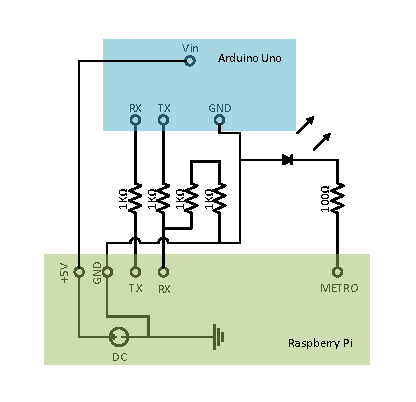
\includegraphics[width=\linewidth/2]{capitulo6/proto_esquema}
		\par\end{centering}
	\smallskip
	\caption{\label{fig:proto_esquema} Esquema de la placa de prueba.}
\end{figure} 

\smallskip

\smallskip

\begin{figure}[H]
	\noindent \begin{centering}
		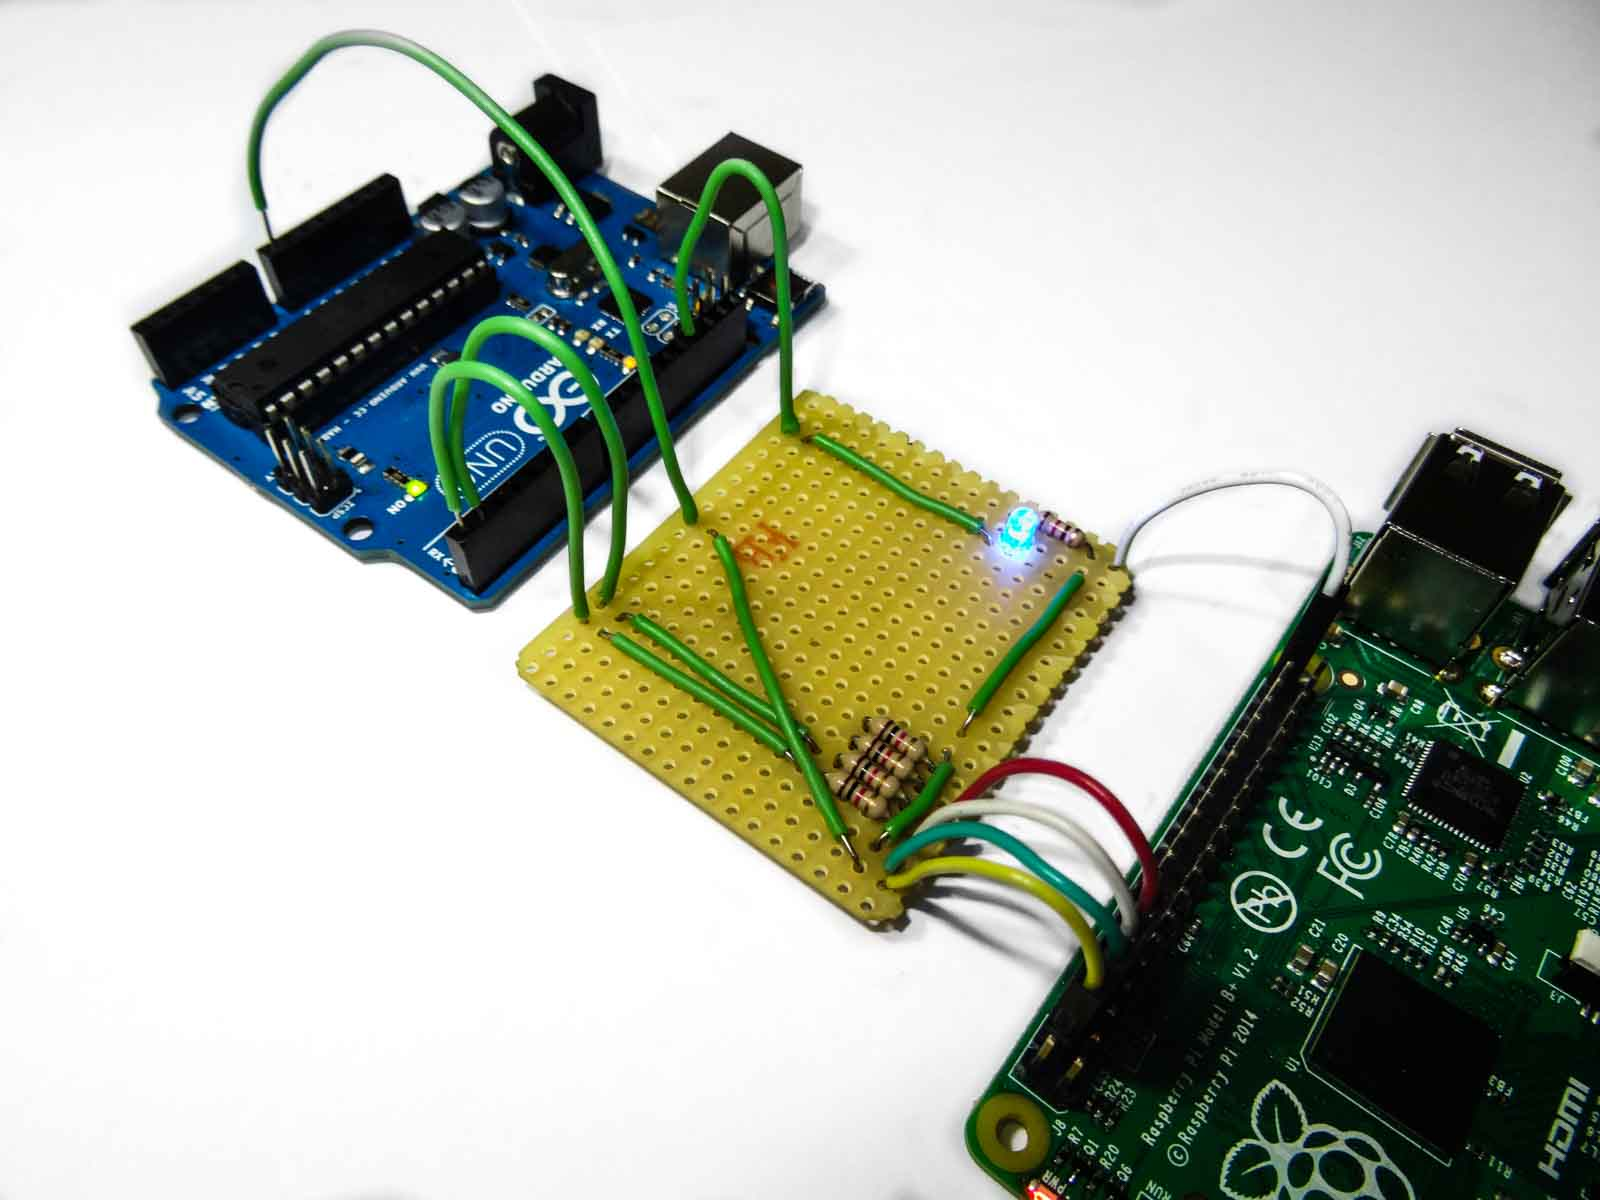
\includegraphics[width=\linewidth*2/3]{capitulo6/proto_uart}
		\par\end{centering}
	\smallskip
	\caption{\label{fig:proto_uart} Placa de prueba.}
\end{figure} 

\smallskip

\subsection{Rendimiento}

\subsubsection{Analizador MIDI}

\smallskip

\begin{figure}[H]
	\noindent \begin{centering}
		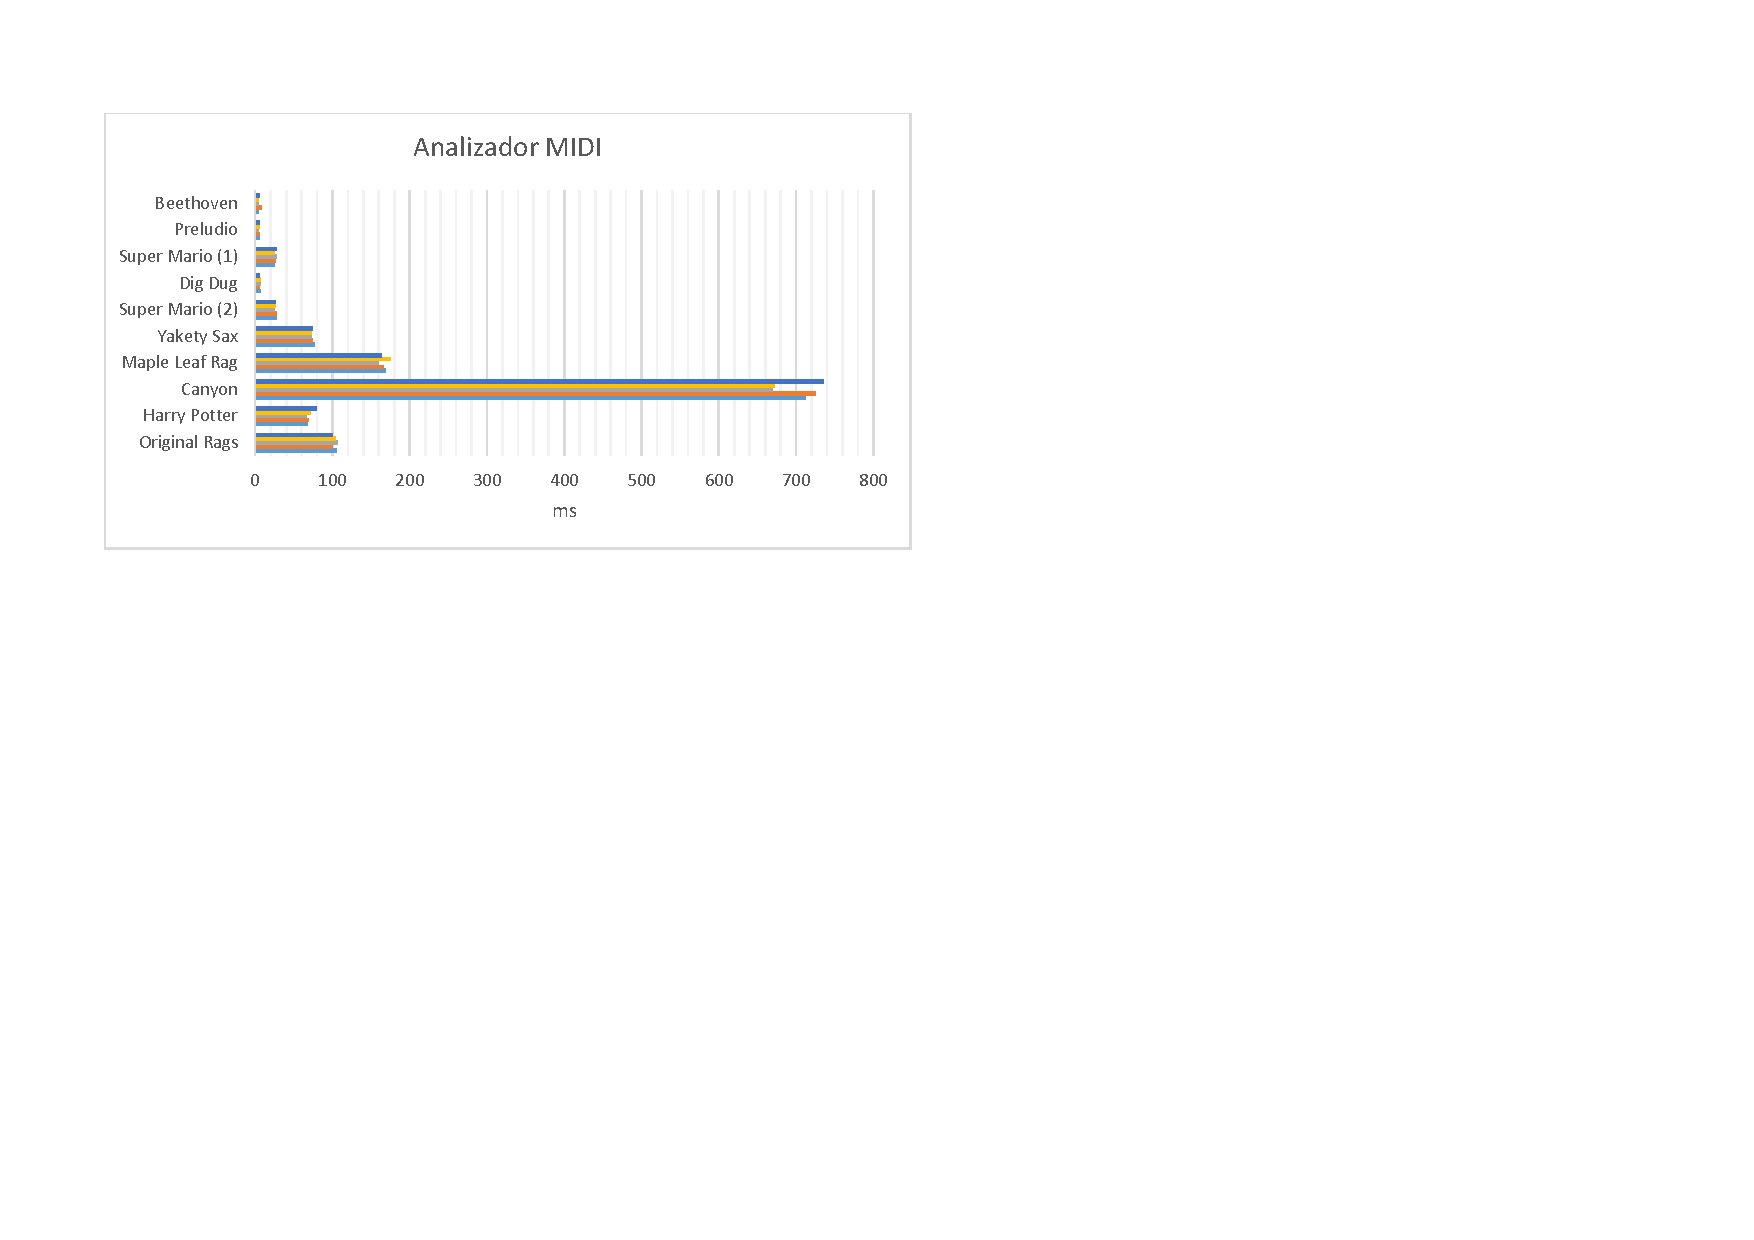
\includegraphics[width=\linewidth*3/4]{capitulo6/lat_midi}
		\par\end{centering}
	\smallskip
	\caption{\label{fig:lat_midi} Tiempo de ejecución del analizador MIDI.}
\end{figure} 

\smallskip

\subsubsection{Planificador}

\smallskip

\begin{figure}[H]
	\noindent \begin{centering}
		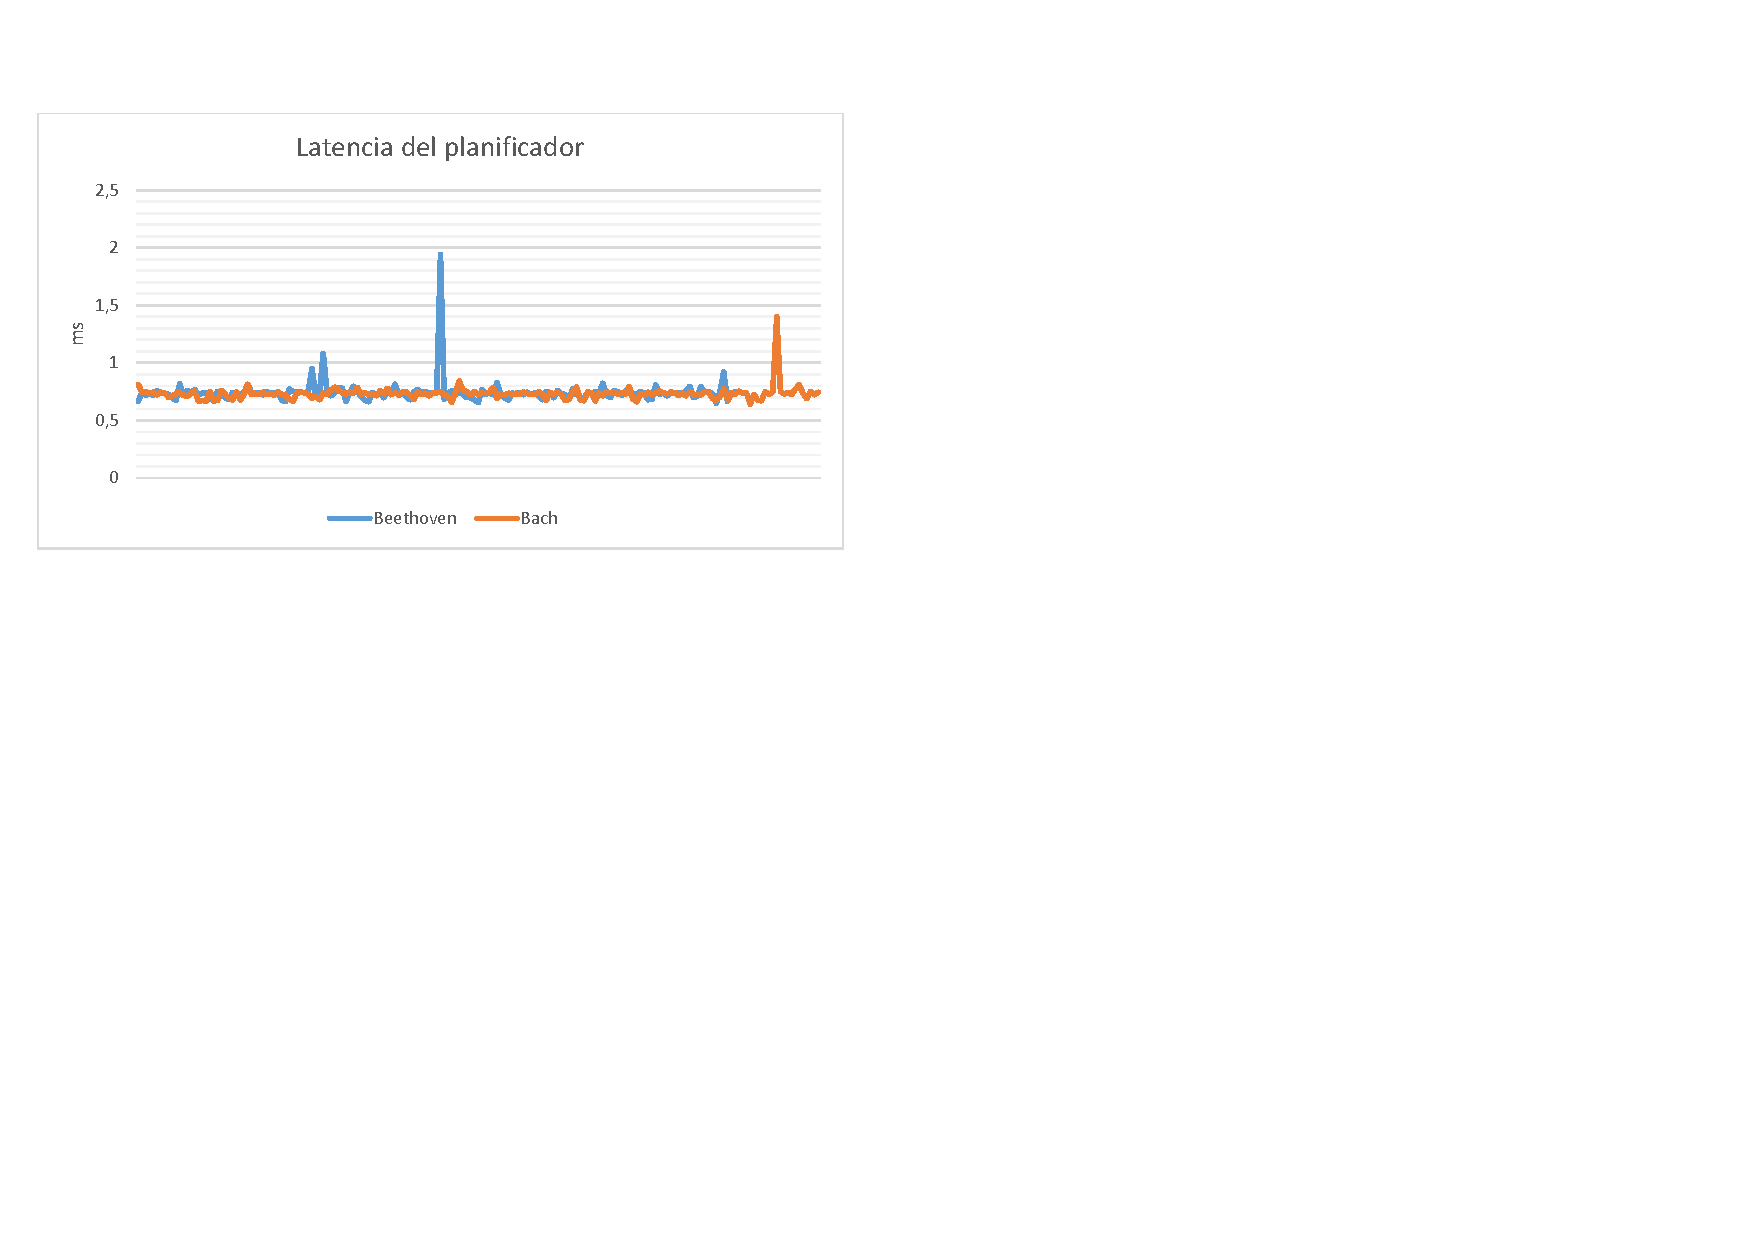
\includegraphics[width=\linewidth*3/4]{capitulo6/lat_sched}
		\par\end{centering}
	\smallskip
	\caption{\label{fig:lat_sched} Tiempo de ejecución del planificador.}
\end{figure} 

\smallskip

\subsubsection{Salida GPIO}

\smallskip

\begin{figure}[H]
	\noindent \begin{centering}
		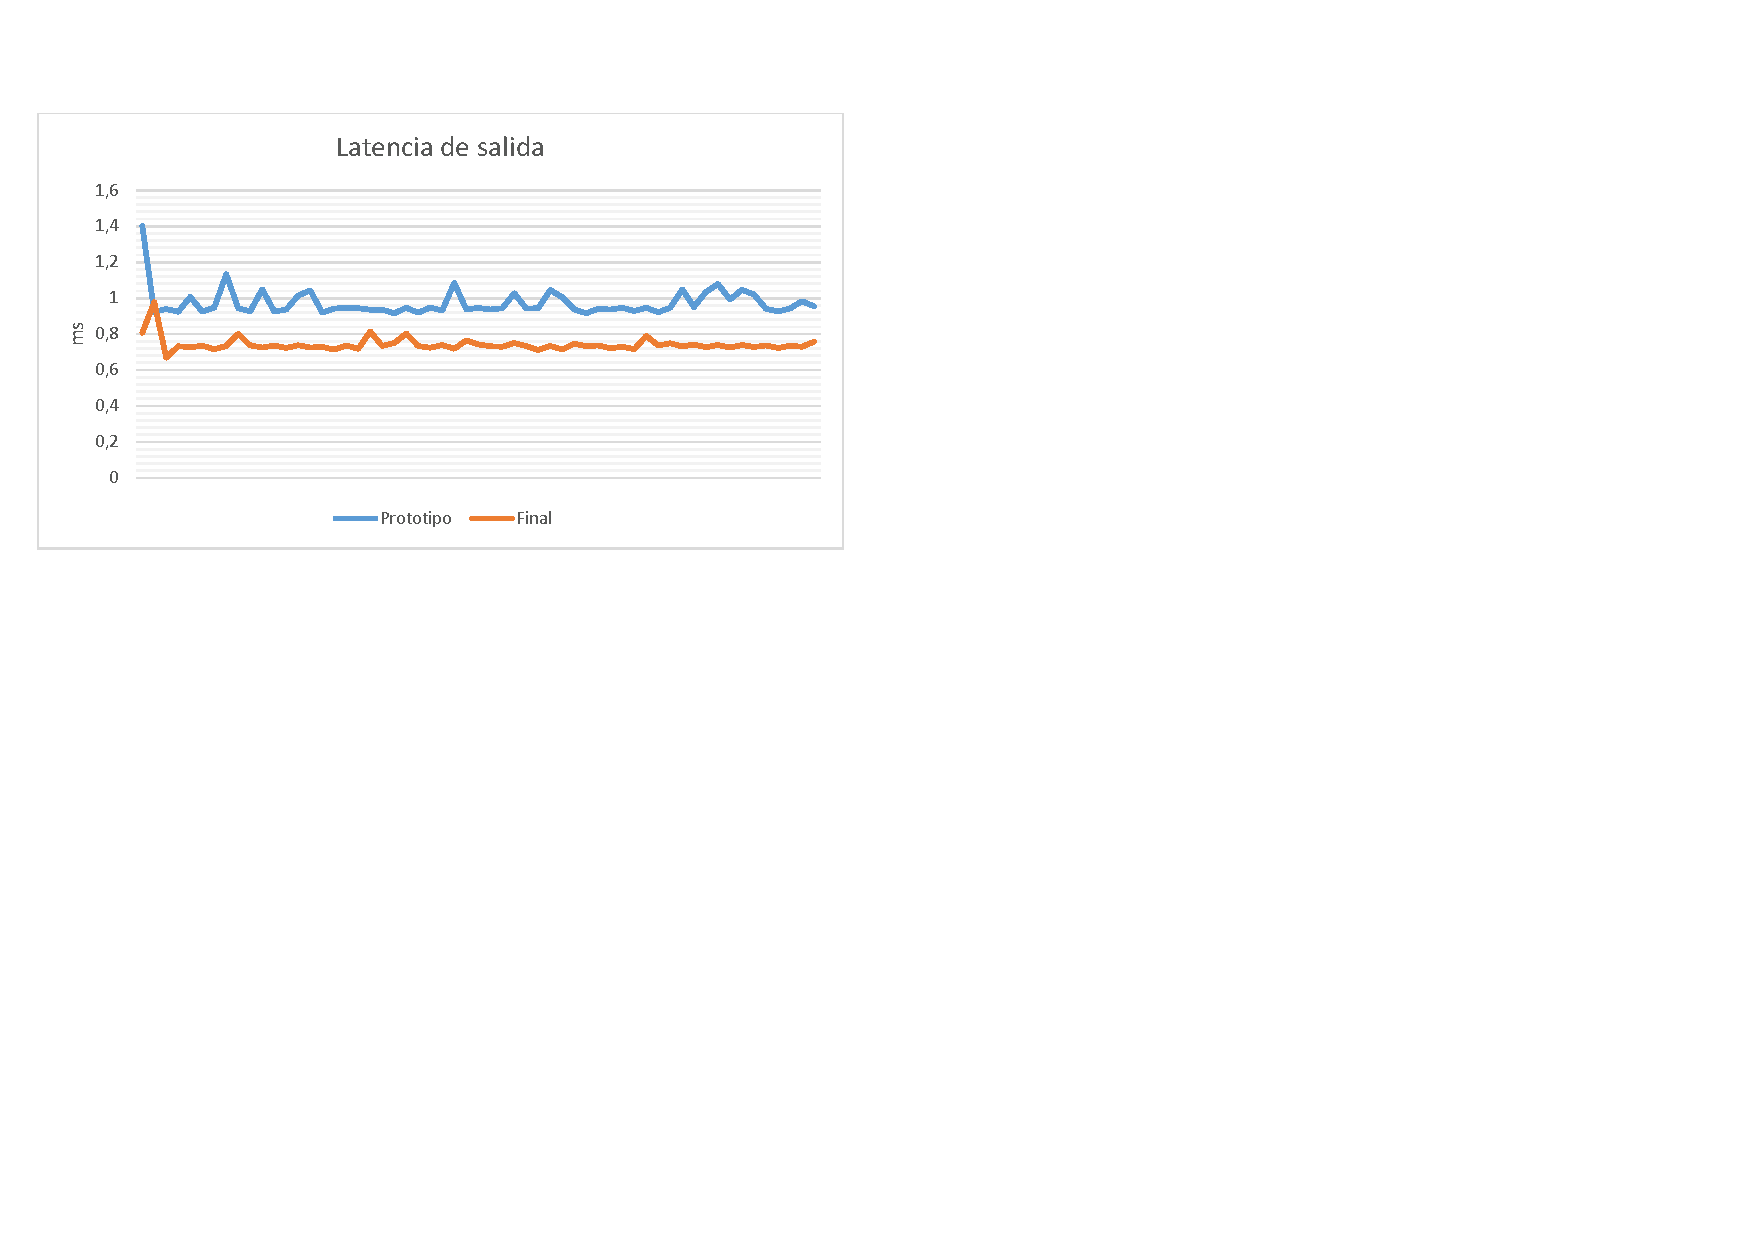
\includegraphics[width=\linewidth*3/4]{capitulo6/lat_gpio}
		\par\end{centering}
	\smallskip
	\caption{\label{fig:lat_gpio} Tiempo de ejecución de la salida a GPIO.}
\end{figure} 

\smallskip

\subsubsection{Aplicaciones auxiliares}

\smallskip

\begin{figure}[H]
	\noindent \begin{centering}
		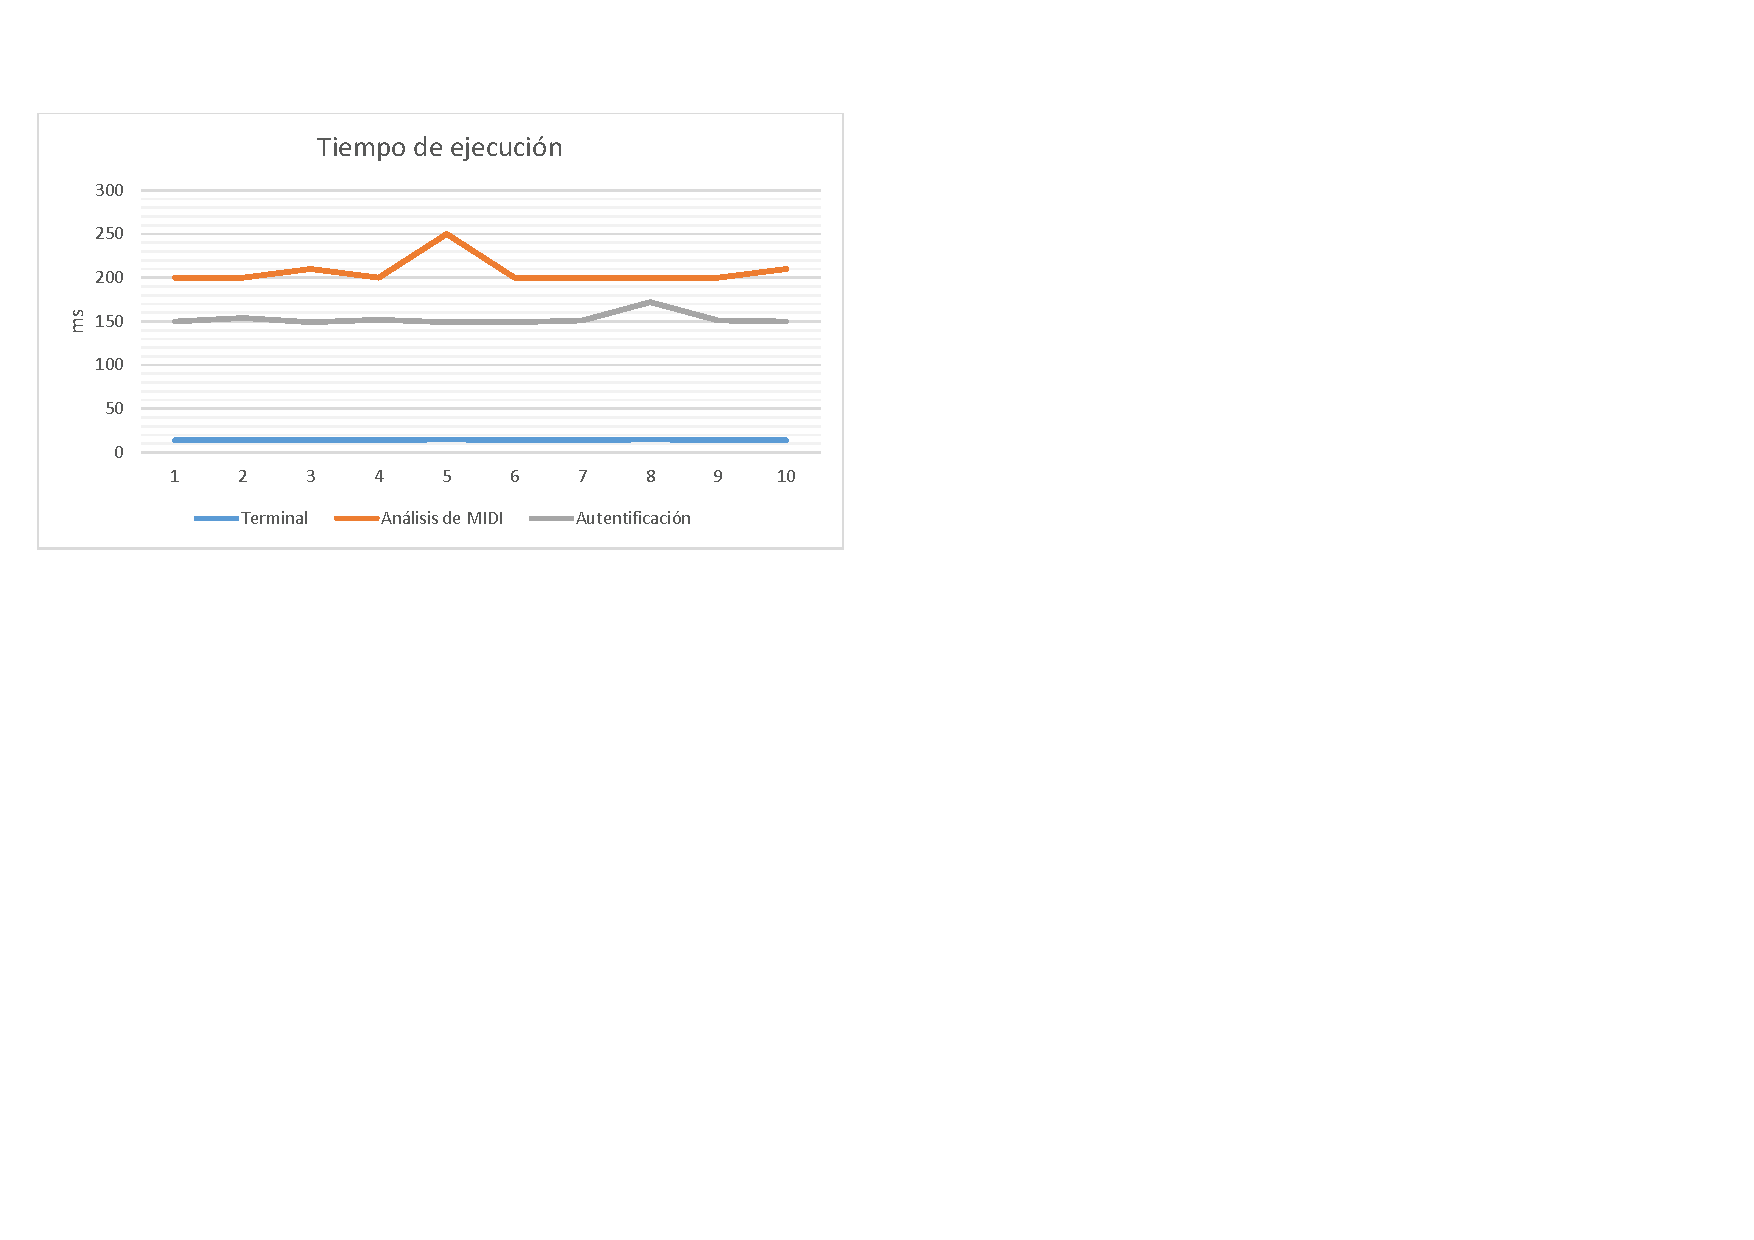
\includegraphics[width=\linewidth*3/4]{capitulo6/ejecucion}
		\par\end{centering}
	\smallskip
	\caption{\label{fig:ejecucion} Tiempo de ejecución de los programas auxiliares.}
\end{figure} 

\smallskip

\section{Interfaz de control}

\subsection{Requisitos}

\subsubsection{Seguridad}

\subsection{Rendimiento}

\smallskip

\begin{figure}[H]
	\noindent \begin{centering}
		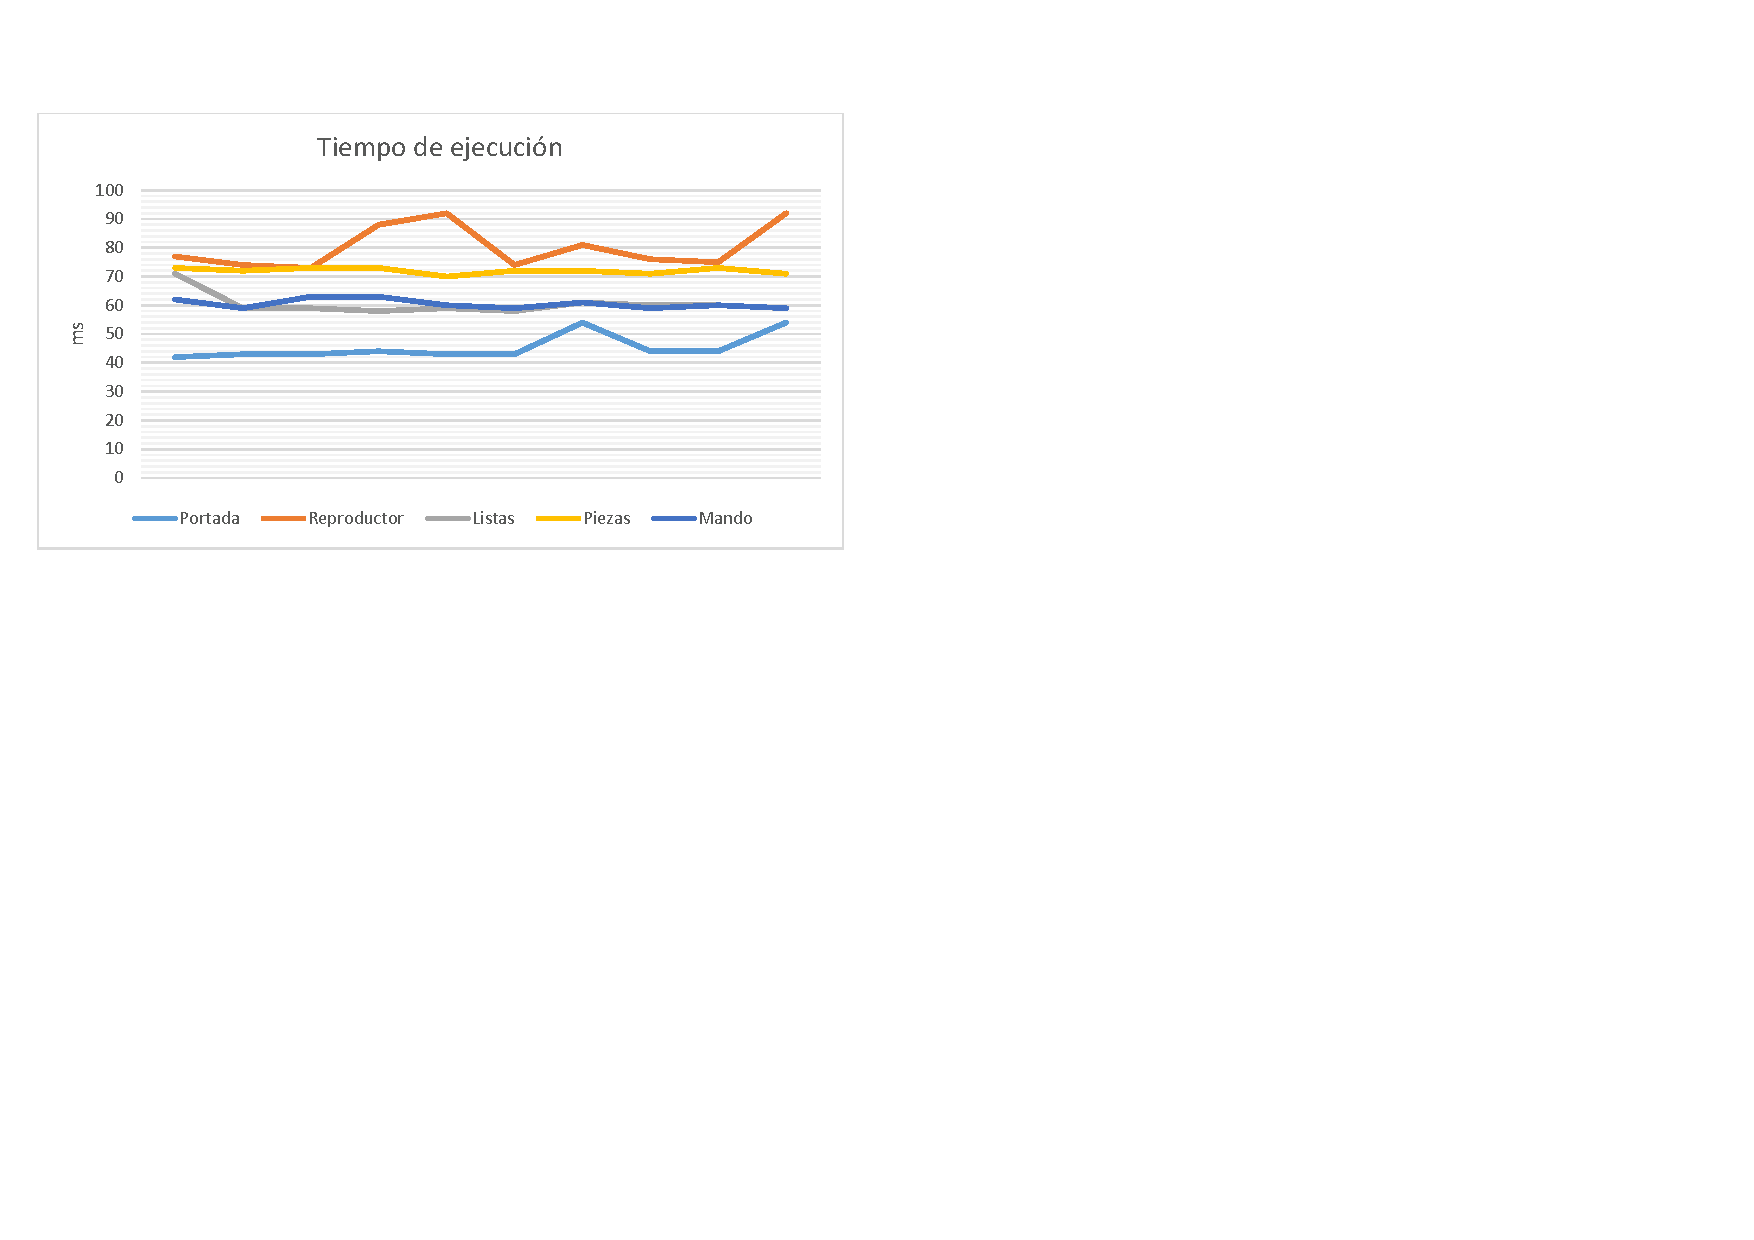
\includegraphics[width=\linewidth*3/4]{capitulo6/ejecucion_web}
		\par\end{centering}
	\smallskip
	\caption{\label{fig:ejecucion_web} Tiempo de ejecución de las vistas.}
\end{figure} 

\smallskip

\section{Prueba sobre la PCB}

\smallskip

\begin{figure}[H]
	\noindent \begin{centering}
		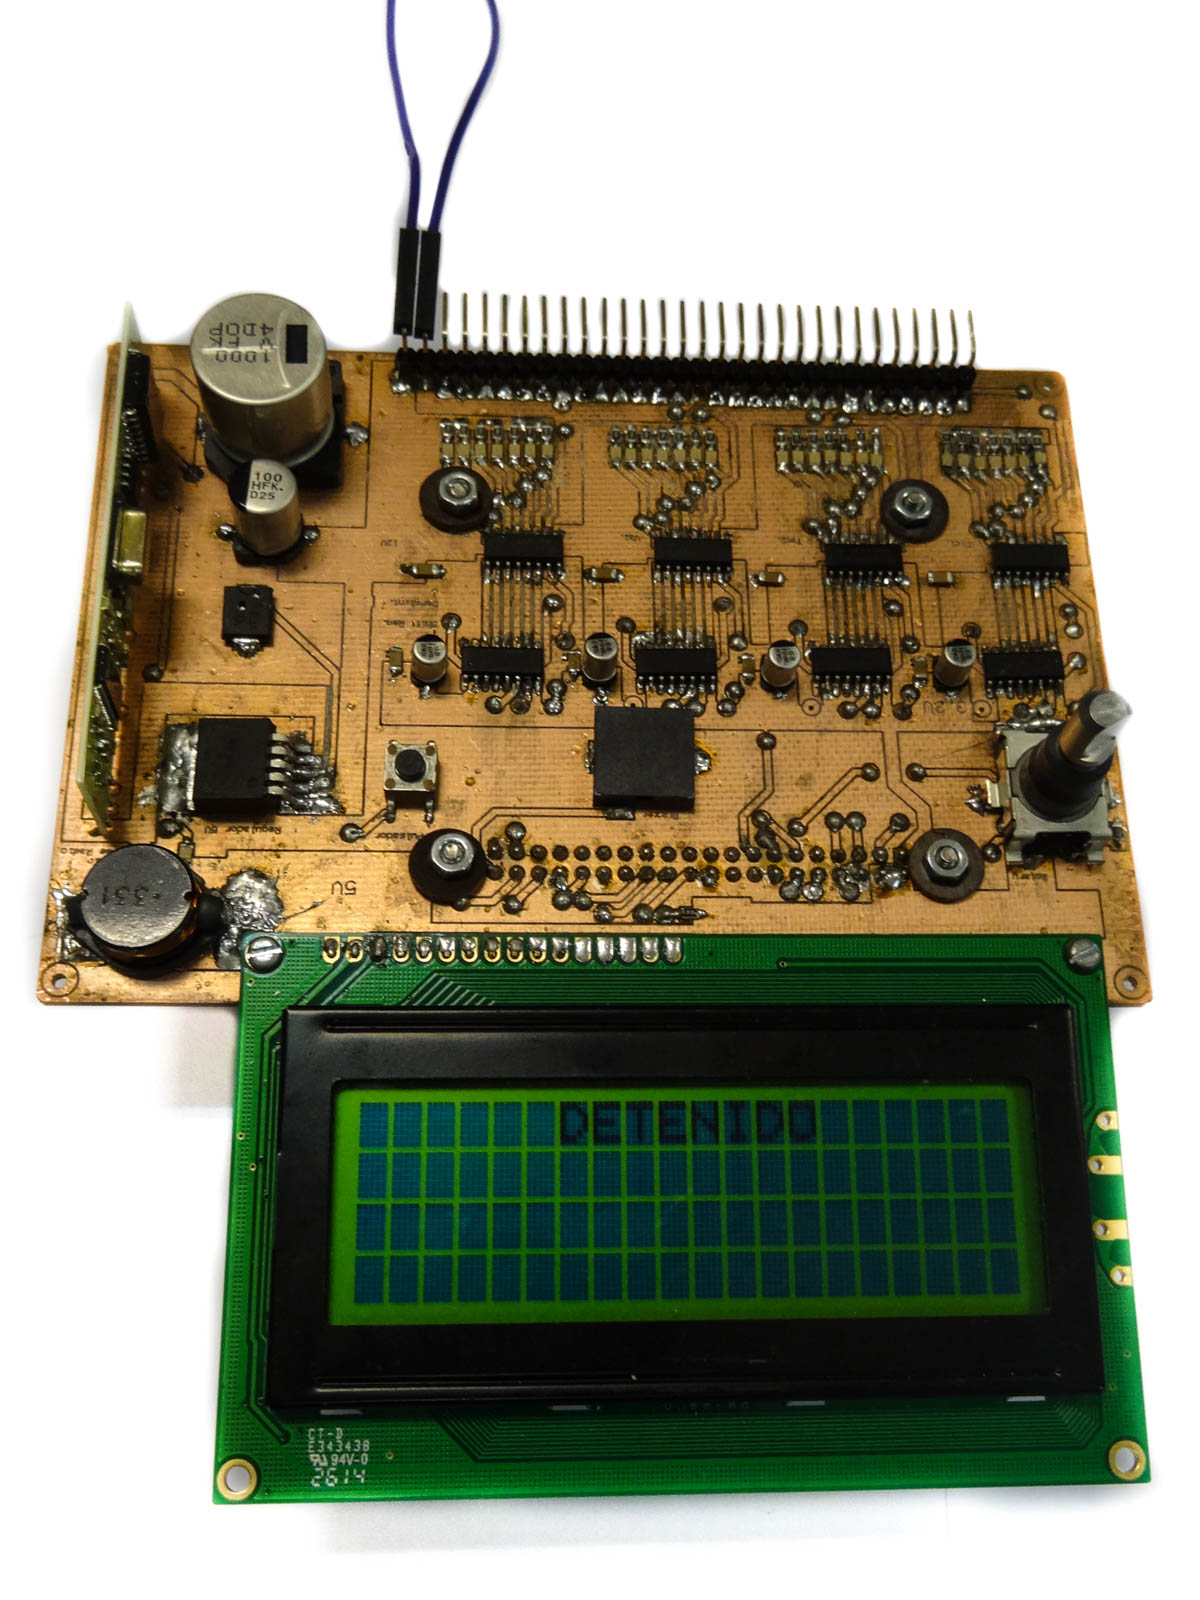
\includegraphics[width=\linewidth*2/3]{capitulo6/pcb}
		\par\end{centering}
	\smallskip
	\caption{\label{fig:pcb} Prototipo hardware.}
\end{figure} 

\smallskip

\subsection{Entrada de datos}

\smallskip

\begin{figure}[H]
	\noindent \begin{centering}
		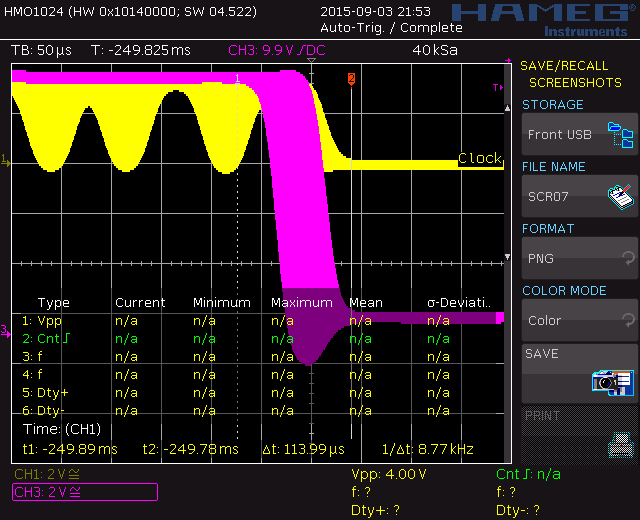
\includegraphics[width=\linewidth*2/3]{capitulo6/osc_pulso}
		\par\end{centering}
	\smallskip
	\caption{\label{fig:osc_pulso} Ancho de pulso.}
\end{figure} 

\smallskip

\smallskip

\begin{figure}[H]
	\noindent \begin{centering}
		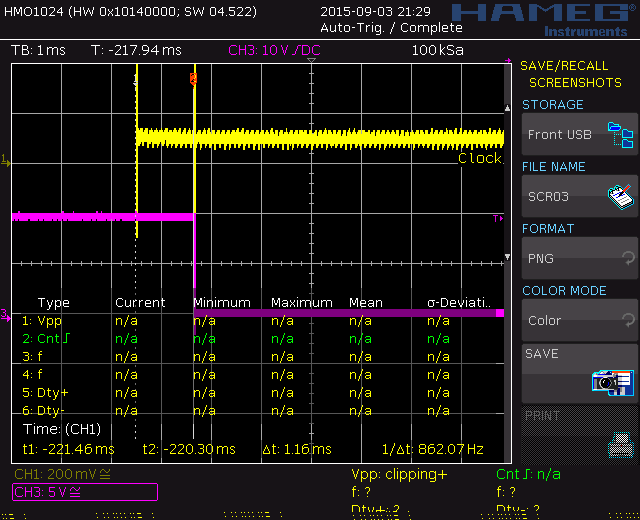
\includegraphics[width=\linewidth*2/3]{capitulo6/osc_nota}
		\par\end{centering}
	\smallskip
	\caption{\label{fig:osc_nota} Tiempo de transmisión de una nota.}
\end{figure} 

\smallskip

\subsection{Modo Ingeniería}

\smallskip

\begin{figure}[H]
	\noindent \begin{centering}
		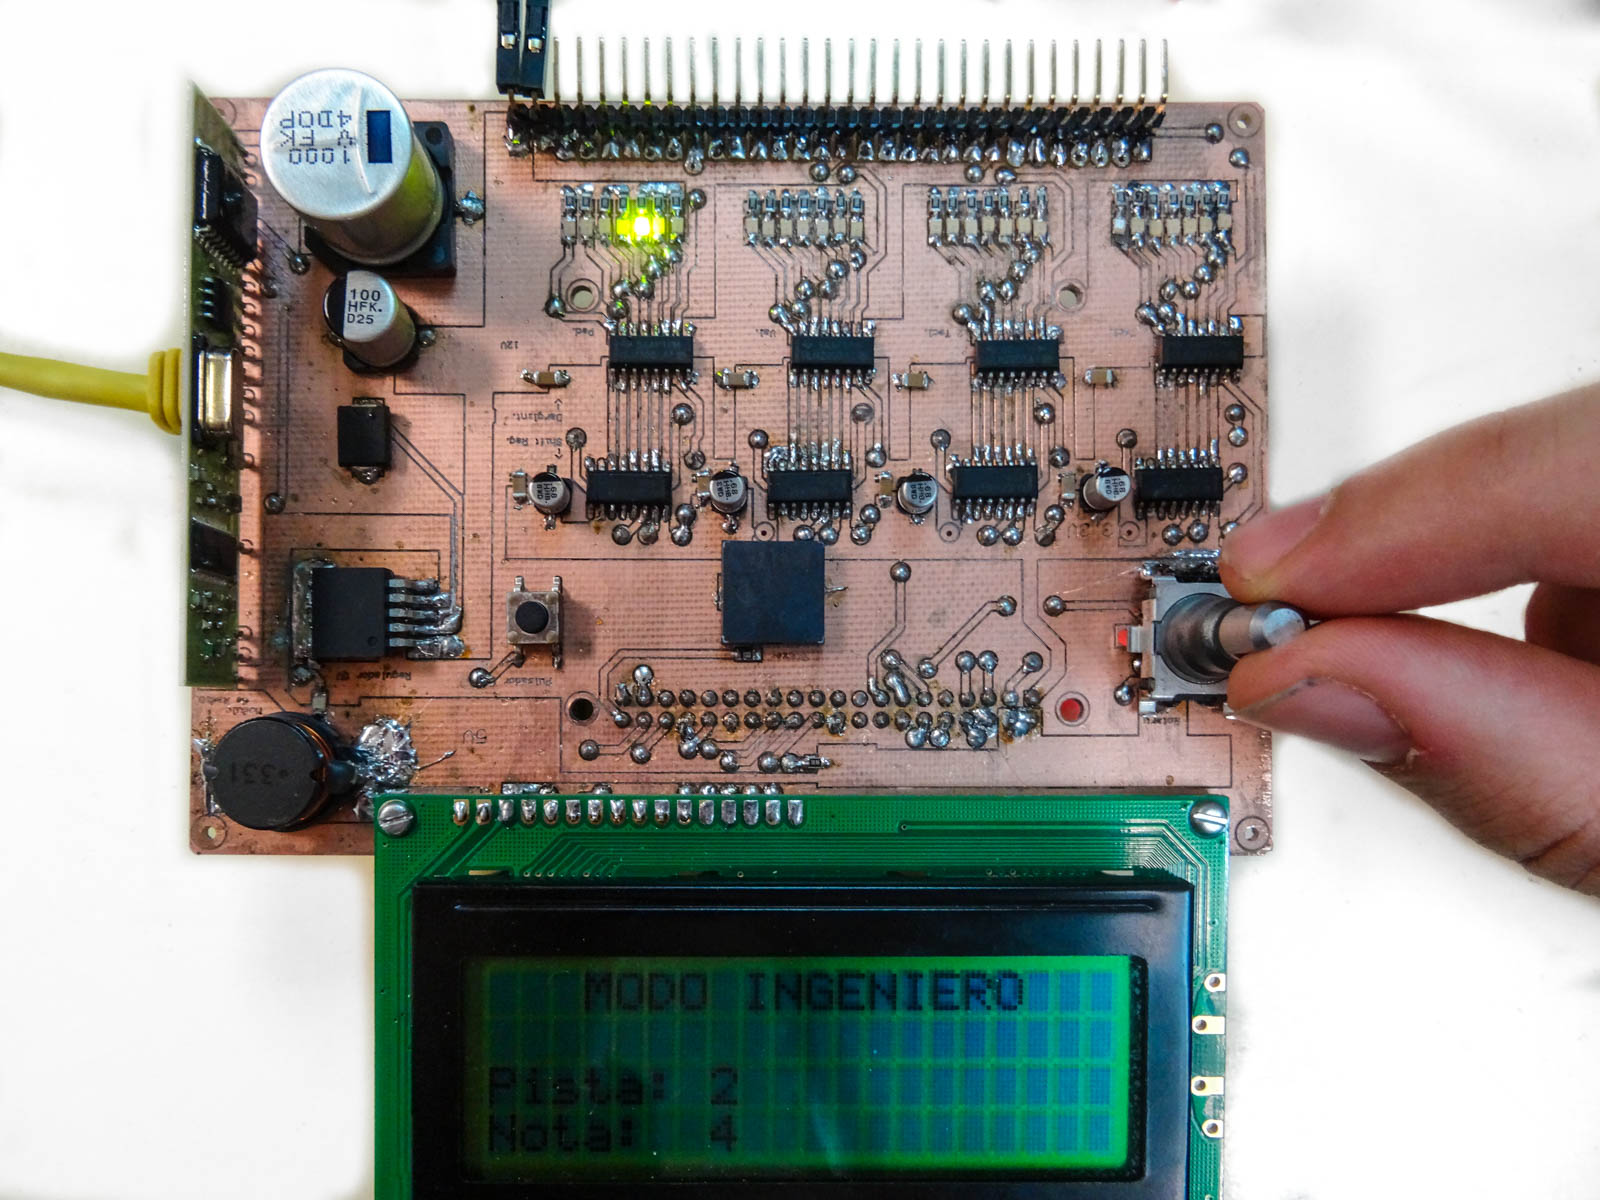
\includegraphics[width=\linewidth*2/3]{capitulo6/pcb_ingeniero}
		\par\end{centering}
	\smallskip
	\caption{\label{fig:pcb_ingeniero} PCB en modo Ingeniería.}
\end{figure} 

\smallskip

\clearpage{\cleardoublepage}
\clearpage{\pagestyle{empty}\cleardoublepage}

